\documentclass[a4paper,oneside,11pt]{memoir}

\usepackage[utf8]{inputenc} % input encoding
\usepackage[T1]{fontenc} % font encoding

\usepackage{graphicx} %to include images/graphics
\usepackage{amsmath,amssymb} %better math type setting
\usepackage{listings} %for source code snippets
\usepackage{textcomp} %for upquote
\usepackage{xcolor} % nice colors (for source code)
\usepackage{pgfgantt}
\usepackage{longtable}
\usepackage{booktabs}


% Graphics and diagrams
\usepackage{tikz}
\usetikzlibrary{shapes.geometric, arrows.meta, positioning, fit, backgrounds, shadows}
 


\renewcommand{\ttdefault}{pcr} % nicer font for source code

% an example configuration of the 'listings' package
\lstset{basicstyle=\ttfamily, 
        keywordstyle=\color{purple}\ttfamily,
        commentstyle=\color{gray}\ttfamily,
        stringstyle=\color{orange}\ttfamily,
        captionpos=b,
        float=tb,
        upquote=true,
}

\chapterstyle{tandh} % configuration of the 'memoir' class


% ── Listing style ────────────────────────────────────────────────
\lstdefinestyle{jsonStyle}{
    basicstyle=\ttfamily\footnotesize,
    backgroundcolor=\color{gray!10},
    frame=single,
    rulecolor=\color{gray!40},
    breaklines=true,
    captionpos=b,
    numbers=left,
    numberstyle=\tiny\color{gray},
    keywordstyle=\color{blue},
    stringstyle=\color{orange!70!black},
    commentstyle=\color{green!50!black}
}


% Custom style for CSV data listings
\lstdefinestyle{csvStyle}{
    backgroundcolor=\color{gray!5},
    basicstyle=\ttfamily\footnotesize,
    breakatwhitespace=false,
    breaklines=true,
    captionpos=b,
    commentstyle=\color{gray},
    frame=single,
    frameround=tttt,
    framesep=5pt,
    keepspaces=true,
    keywordstyle=\color{blue!70!black}\bfseries,
    morekeywords={timestamp,mmsi,name,ship_type,lat,lon,speed_kn,course_deg},
    numbers=left,
    numbersep=10pt,
    numberstyle=\tiny\color{gray},
    rulecolor=\color{gray!40},
    showspaces=false,
    showstringspaces=false,
    tabsize=2,
    xleftmargin=20pt
}
 
% ── TikZ styles ──────────────────────────────────────────────────
\tikzset{
    block/.style={
        rectangle, draw, fill=blue!10,
        text width=3.2cm, align=center,
        minimum height=1.0cm, rounded corners=3pt,
        drop shadow
    },
    blockRed/.style={
        rectangle, draw, fill=red!10,
        text width=3.2cm, align=center,
        minimum height=1.0cm, rounded corners=3pt,
        drop shadow
    },
    blockGreen/.style={
        rectangle, draw, fill=green!10,
        text width=3.2cm, align=center,
        minimum height=1.0cm, rounded corners=3pt,
        drop shadow
    },
    blockGray/.style={
        rectangle, draw, fill=gray!10,
        text width=3.2cm, align=center,
        minimum height=1.0cm, rounded corners=3pt,
        drop shadow
    },
    arrow/.style={-{Stealth[length=2mm]}, thick},
    dasharrow/.style={-{Stealth[length=2mm]}, thick, dashed},
    label/.style={font=\footnotesize\ttfamily, align=center}
}
 
% ================================================================

%
% The actual document starts here
%
\begin{document}

\begin{titlingpage}
\thispagestyle{empty}

\centering
  \vspace*{6.5em}

  \textsc{\textbf{\huge A Distributed Simulation Sandbox for Decentralized 
  Control Algorithms in Marine Drone Swarms}}
  \vspace{4.5em}

  \textsc{\Large
    \setlength{\tabcolsep}{12pt}
    \begin{tabular}[h]{lr}
      %blablabla
      \\[.4\onelineskip]
      Alan Tomasz Bejnarowicz   &  4132829
    \end{tabular}
  }

  \vspace{5em}
  \large
  % 
  % Adjust the type of thesis and education here
  % 
  % Bachelor Project in Engineering (Robot Systems)
  % Bachelor Project in Engineering (Robot Systems)
  Masters Project in Engineering (Drones and Autonomous Systems)
  
  %Supervisor: Louise Lind\\
  %Co-supervisor: Klaus Kristensen
  Supervisor: Xiaofeng Xiong
  \normalsize
  \vspace{2em}
  \\[1em]
  \today
  %June 1887


  \vspace{9em}
  
\includegraphics[width=.5\textwidth]{sdu_logo}
  
  \vspace{3em}
  The Maersk Mc-Kinney Moeller Institute

  \medskip
  University of Southern Denmark
  
   %Word count: 1234
\end{titlingpage}


\cleardoublepage

\frontmatter

% abstract 
\begin{abstract}
\sloppy
  This thesis proposes the design and implementation of a 
    high-performance 
      simulation sandbox for developing and testing decentralized control 
      algorithms for autonomous sailing drone swarms. 
      The core of the project is a simulation environment.
      The simulator models key marine dynamics, including wind and sea conditions, 
      and incorporates virtual sensors, 
      along with inter-drone communication channels.

      \vspace{1em}

      The motivation for this work is its application in maritime search and rescue (SAR).
      By leveraging a swarm of inexpensive, autonomous drones, the 
      time to locate a drowning victim can be significantly reduced, dramatically 
      increasing the chances of survival. 

      \vspace{1em}

      As of October 2025, there are no known existing solutions that combine simulation,
      SITL/HITL capabilities, and decentralized control for marine drone swarms,
      making this project a pioneering effort in autonomous maritime robotics.
      Existing tools tend to target aerial drones or are general-purpose robotics
      simulators and require heavy modification to support marine dynamics and
      large-scale swarm experiments. A related project is YARA\cite{YARA}, a
      Gazebo-based sailing drone simulator, but it lacks SITL/HITL support and is
      not optimized for extensive swarm simulations.

      \vspace{1em}

      This work will implement a cross-robot communication channel model with
      signal attenuation, delays, and packet dropouts. The simulator will provide
      sensor models for IMU, GPS, and AIS (Automatic Identification System) 
      and will support replaying historical AIS datasets to
      populate and simulate real vessel traffic within the environment. The
      platform will also allow isolating and instantiating independent swarms
      to enable large-scale training and
      evaluation of genetic algorithms and neural-network based controllers.
      \vspace{1em}

      The simulator will be validated through a series of experiments, including
      benchmarking decentralized control algorithms for formation keeping,
      collision avoidance, and cooperative search tasks. The performance of the
      simulator will be assessed based on its computational efficiency, scalability,
      and fidelity in replicating real-world marine conditions.

      \vspace{0.4em}
      \begin{center}
        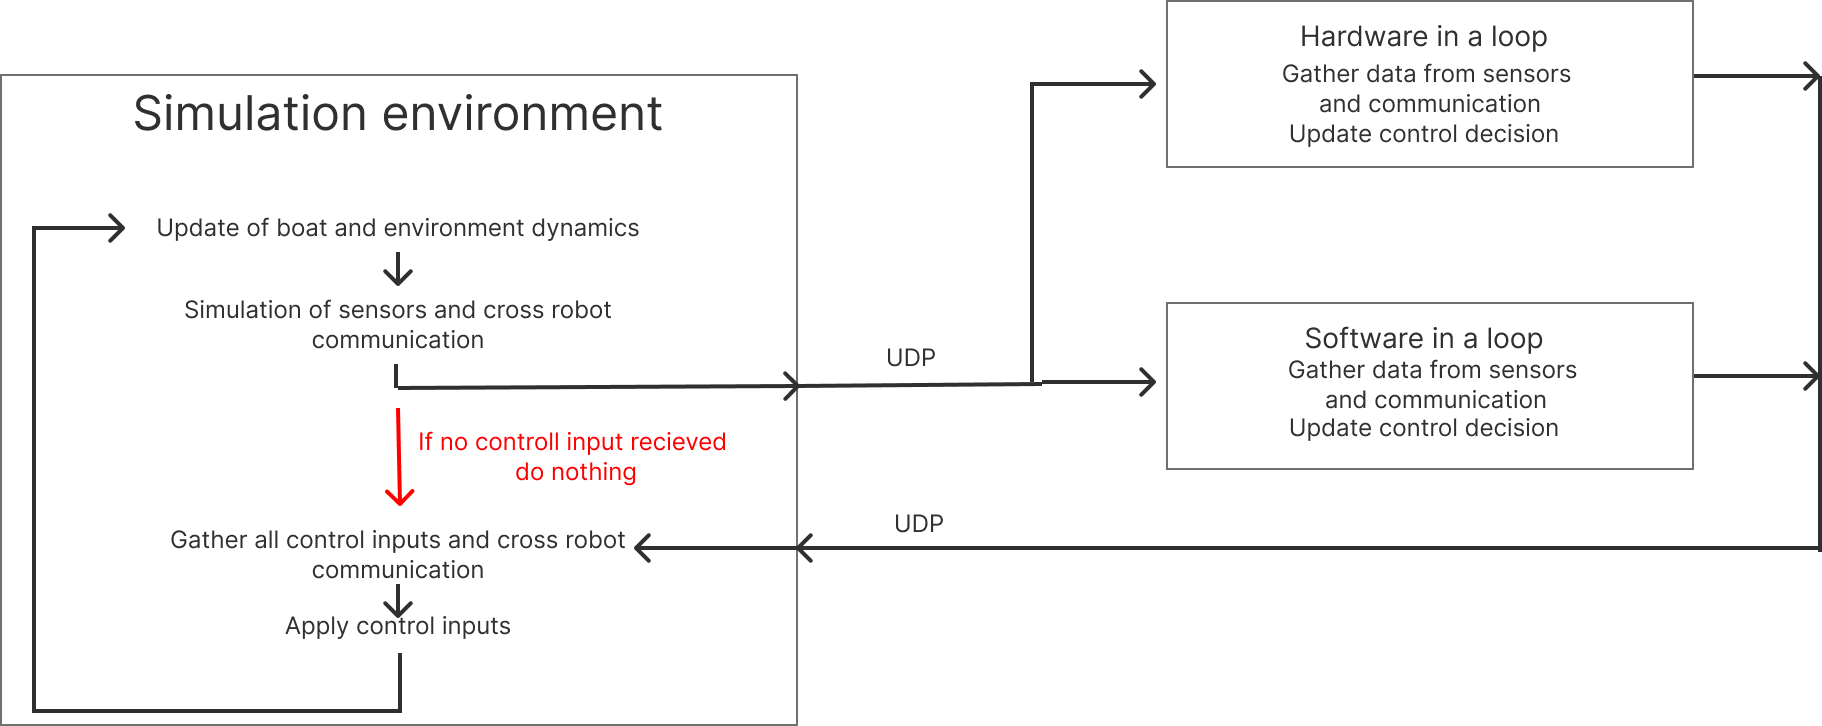
\includegraphics[width=0.7\textwidth]{images/simulation_schematic.png}
        
        {\small\textit{Proposed simulation dataflow.}}
      \end{center}

\end{abstract}


\begin{center}
\textsc{Work schedule / Gantt chart}
\end{center}

\vspace{1cm}

\begin{center}

\scalebox{0.8}{%
\begin{ganttchart}[
        hgrid,
        vgrid,
        x unit=1.1cm,
        y unit chart=0.9cm,
        title height=1,
        bar height=0.55,
        group height=0.7,
        bar/.append style={fill=blue!50},
        group/.append style={fill=gray!50},
        milestone/.append style={fill=red!70},
        % Make labels readable: use dark text for left labels
        bar label font=\small\color{black},
        bar label node/.append style={align=center, text=black},
        group label font=\small\color{black},
        group label node/.append style={text=black},
        milestone label font=\small,
        milestone label node/.append style={right=2mm}
]{1}{9}

% Titles
\gantttitle{MSc Thesis Work Plan}{9} \\
\gantttitle{2025}{3}
\gantttitle{2026}{6} \\
\gantttitle{Oct}{1}
\gantttitle{Nov}{1}
\gantttitle{Dec}{1}
\gantttitle{Jan}{1}
\gantttitle{Feb}{1}
\gantttitle{Mar}{1}
\gantttitle{Apr}{1}
\gantttitle{May}{1}
\gantttitle{Jun}{1} \\

% Tasks
\ganttgroup{Literature Review \& Background \& Initial work}{1}{3} \\

\ganttbar[
        bar/.append style={fill=green!60}
]{Problem Definition \& Requirements}{2}{4} \\

\ganttbar{System Design}{4}{5} \\

\ganttbar[
        bar/.append style={fill=orange!70}
]{Implementation (Simulator / Prototype)}{4}{8} \\

\ganttbar[
        bar/.append style={fill=orange!70}
]{Implementation of HIL and STIL}{6}{8} \\

\ganttbar[
        bar/.append style={fill=violet!60}
]{Collection of AIS data}{7}{8} \\


\ganttbar{Implementation of swarm algorithm}{6}{8} \\

\ganttbar{Experiments \& Evaluation}{7}{9} \\

\ganttbar[
        bar/.append style={fill=violet!60}
]{Thesis Writing}{5}{9} \\

\ganttmilestone{Thesis Submission}{9}

\end{ganttchart}%
} % end resizebox

\end{center}

\noindent\rule{\linewidth}{0.4pt}\par

\cleardoublepage



%\tableofcontents

\mainmatter

%
% We have one file per chapter:
%

% Example citation to avoid bibliography error
\nocite{*}

% Introduction chapter in 'chap-introduction.tex'
%\chapter{Introduction}
\label{chap:introduction}

Ever since the development of Robots, developers have been questioning how to combine them with machine learning.


% Background chapter in 'chap-background.tex'
%\input{chap-background}

% ...


\section{From YARA Sim to High-Performance Swarm Environments}

Projects like YARA (Yet Another Robotic Actuator/Sailing Simulator) have laid the groundwork using Gazebo to model sailing dynamics, the shift toward autonomous drone swarms requires a leap in both scale and technical sophistication.
This work explores the transition from general-purpose sailing simulators to a specialized, high-performance sandbox designed for decentralized control.


The most significant departure from the YARA framework is the inclusion of SITL (Software-in-the-Loop) and HITL (Hardware-in-the-Loop) capabilities. This ensures that the decentralized algorithms developed in the sandbox aren't just theoretically sound—they are ready for deployment on physical hardware. By bridging the gap between a high-fidelity marine physics engine and real-world flight/sailing controllers, this project moves autonomous maritime robotics from the lab to the ocean.

\section{Drone Ship Physics Model }

Very important part of my project is to have a good physics model of the drone ship. 
That model will be used to simulate IMU and GPS sensor readings, as well as to provide a realistic environment for testing control algorithms.

First step is to model the buoyancy of the ship. The ship will be modeled as a rigid body with a certain mass, width, length, and draft. Currently model does not assume any particular shape for the ship, but it will be important to consider the shape in future iterations to improve the accuracy of the model. The buoyancy force will be calculated based on the 4 points of the ship: the bow, stern, port, and starboard. The buoyancy force will be calculated as the weight of the displaced water, which is equal to the volume of the submerged part of the ship multiplied by the density of water and gravity. 

Same points will be used to calculate the wave drag force. In each of 4 points there is a wave drag force acting in the normal direction to the surface of the water. Forces are scaled to the size of the ship. 

This approach captures the essential physics of the problem while keeping the model computationally efficient. Placement of these points is visible in the figure below
\ref{fig:ship_buoyancy_points}.


That model will be used to simulate the motion of the ship in response to control inputs and environmental forces. 


\begin{figure}[htbp]
    \centering
    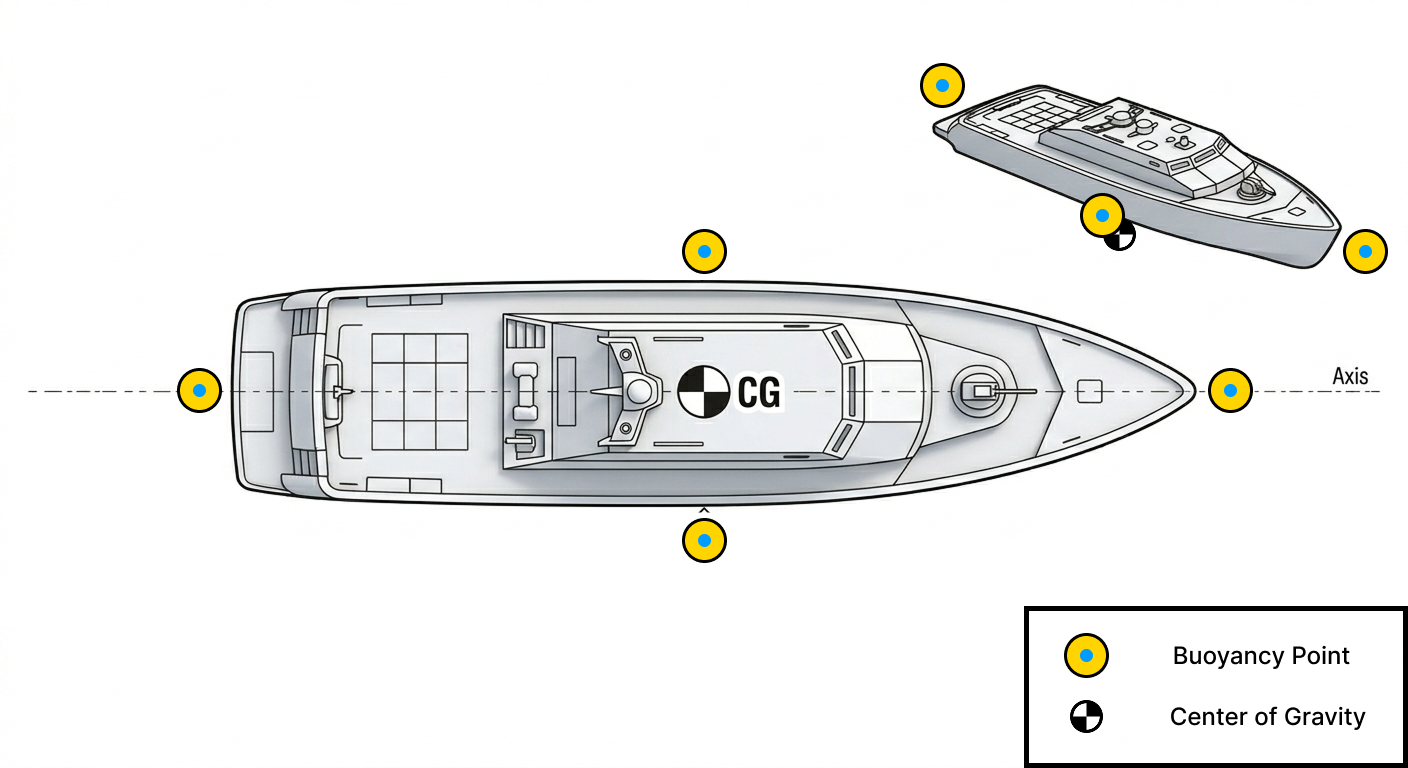
\includegraphics[width=0.8\textwidth]{images/ship_buoyancy.png}
    \caption{Ship buoyancy model diagram.}
    \label{fig:ship_buoyancy_points}
\end{figure}

\section{Wave Physics Model }

The sea surface height $\eta(x, z, t)$ is modeled as a superposition of multiple sinusoidal components, mimicking a simplified Gerstner Wave and following Pierson-Moskowitz spectrum. The total displacement at any point $\mathbf{p}$ is the sum of $n$ wave harmonics:

\begin{equation}
\eta(\mathbf{p}, t) = \sum_{i=1}^{n} A_i \cdot \sin(\mathbf{k}_i \cdot \mathbf{p}_x + \omega_i t) \cdot \cos(\mathbf{k}_{i,z} \cdot \mathbf{p}_z \cdot \phi + \omega_i t)
\end{equation}


Where: $A_i$ is the amplitude of the $i$-th harmonic. $\mathbf{k}_i$ is the wave vector (determining frequency and direction). $\omega_i$ is the angular frequency (phase speed). $\phi$ is a directional interference constant (set to $0.8$ in this model to avoid perfect symmetry).The implementation categorizes these into three distinct scales:
Primary Swells: Low frequency, high amplitude (e.g., $f=0.02, A=0.8$).
Turbulent Mid-levels: Moderate frequency for sea-state texture.
Capillary Ripples: High frequency, low amplitude for surface detail.
Values used in simulation are visible in table \ref{tab:wave_parameters}.



\begin{figure}[htbp]
    \centering
    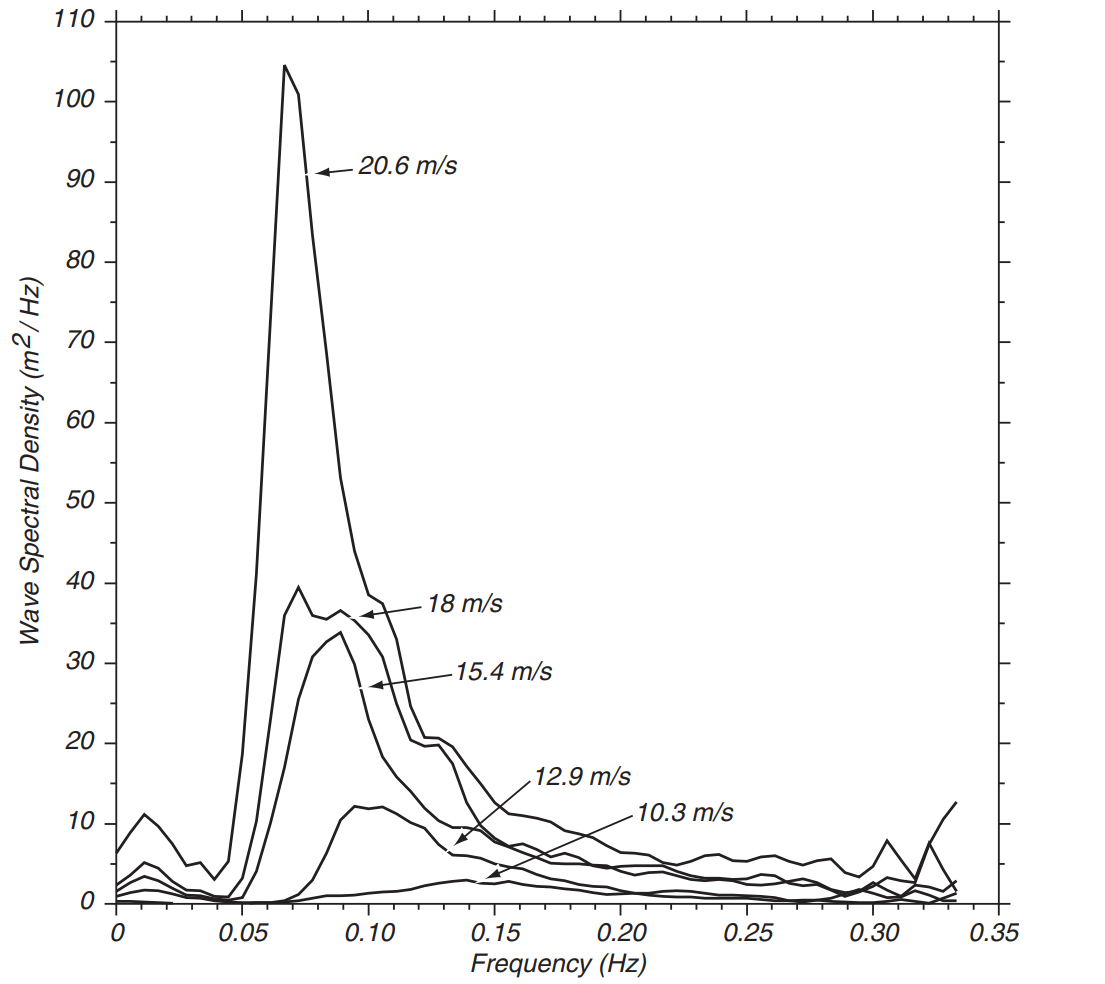
\includegraphics[width=0.7\textwidth]{images/MoskowitzSpectra.png}
    \caption{Wave spectra for different wind speeds according to Moskowitz (1964). \cite{alves2003revisiting}}
    \label{fig:moskowitz_spectra}
\end{figure}


\begin{table}[h]
\centering

\caption{Spectral Parameters for Procedural Wave Synthesis}
\label{tab:wave_parameters}
\begin{tabular}{lccc}
\toprule
\textbf{Wave Category} & \textbf{Frequency} ($f$) & \textbf{Speed} ($v$) & \textbf{Amplitude} ($A$) \\ 
\midrule
Primary Swell 1        & 0.02 Hz                 & 1.2 m/s             & 0.80 m                          \\
Primary Swell 2        & 0.04 Hz                 & 1.5 m/s             & 0.50 m                          \\
Mid-level Turbulence   & 0.10 Hz                 & 2.2 m/s             & 0.20 m                          \\
Secondary Turbulence   & 0.18 Hz                 & 1.8 m/s             & 0.15 m                          \\
Surface Micro-Ripple   & 0.45 Hz                 & 3.0 m/s             & 0.05 m                          \\
Capillary Ripple       & 0.80 Hz                 & 4.2 m/s             & 0.02 m                          \\ \bottomrule
\end{tabular}
\end{table}



To calculate buoyancy forces, the surface normal $\mathbf{\hat{n}}$ must be derived. Rather than analytical differentiation, which becomes computationally expensive as $n$ increases, a Finite Difference Method is used. By sampling the height at four orthogonal offsets around a point $\mathbf{p}$, the slope is determined:

\begin{align}
\frac{\partial \eta}{\partial x} \approx \frac{\eta(x-\epsilon, z) - \eta(x+\epsilon, z)}{2\epsilon}\\
\frac{\partial \eta}{\partial z} \approx \frac{\eta(x, z-\epsilon) - \eta(x, z+\epsilon)}{2\epsilon}
\end{align}


The resulting normal vector is:

\begin{equation}
\mathbf{\hat{n}} = \text{normalize}\left( \frac{\partial \eta}{\partial x}, 1.0, \frac{\partial \eta}{\partial z} \right)
\end{equation}

This is later used in Physics Model to calculate Wave-Slope Dynamics.


\begin{figure}[htbp]
    \centering
    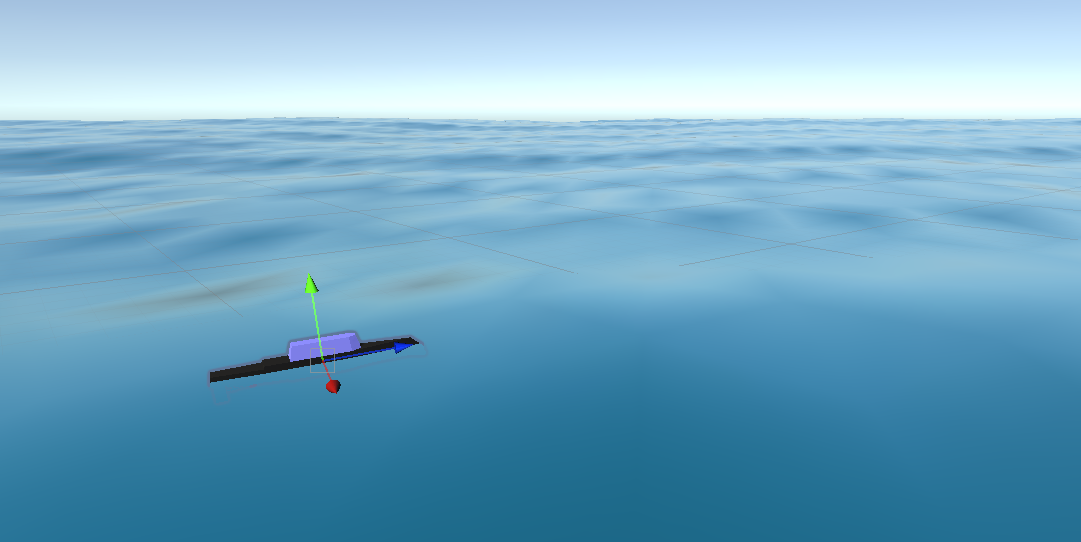
\includegraphics[width=0.8\textwidth]{images/waves_system2.png}
    \caption{Waves simulation resoults.}
    \label{fig:waves_model}
\end{figure}

\subsection{Introduction to Sensor Simulation}

To bridge the gap between a high-fidelity physics environment and autonomous control logic, the simulation must provide synthetic data that replicates the characteristics of physical hardware. In a real-world marine deployment, the vessel’s State Estimation is derived from a suite of diverse sensors, each with its own coordinate frame, sampling rate, and error profile.The virtual sensor suite developed for this simulator focuses on three primary components:

\begin{enumerate}
    
    \item \textbf{Global Positioning System (GPS):} Provides low-frequency absolute positioning and Ground Speed.
    
    \item \textbf{Inertial Measurement Unit (IMU):} A high-frequency 6-axis sensor measuring proper linear acceleration ($\mathbf{a}$) and angular velocity ($\mathbf{\omega}$).
    
    \item \textbf{Digital Compass/Magnetometer:} Provides a heading reference ($\psi$) relative to the magnetic North.

\end{enumerate}

The following sections detail the mathematical transformation of "Ground Truth" data—the perfect state vectors provided by the physics engine—into noisy, biased, and discretized signals. This approach ensures that control algorithms, such as PID loops or Extended Kalman Filters (EKF), are tested against the same signal degradation they would encounter at sea.





\subsection{Global Positioning System (GPS) Simulation}

The GPS module simulates a receiver providing absolute geographic coordinates $(\phi, \lambda)$. Because the simulation environment utilizes a flat Cartesian grid, a conversion between Euclidean distance and Geodetic displacement is required. A reference origin, $\text{GPS}_{ref}$, is defined with a known Latitude $\phi_0$ and Longitude $\lambda_0$. The current position is derived by projecting the ship's relative displacement $(\Delta x, \Delta z)$ onto the Earth's ellipsoidal surface (WGS84).The change in latitude $\Delta \phi$ is calculated as:

\begin{equation}
    \Delta \phi = \frac{\Delta z}{R_M}
\end{equation}

where $R_M$ is the meridian radius of curvature ($\approx 111,111$ m per degree).The change in longitude $\Delta \lambda$ depends on the current latitude, as the meridians converge toward the poles:

\begin{equation}
    \Delta \lambda = \frac{\Delta x}{R_E \cos(\phi_0)}
\end{equation}

where $R_E$ is the Earth's equatorial radius.The final simulated coordinates incorporate a lower sampling frequency ($f_s = 5-10$ Hz) and horizontal dilution of precision (HDOP) modeled as Gaussian noise $\eta_{gps}$:

\begin{align}
    \phi_{sim} &= \phi_0 + \Delta \phi + \eta_{\phi} \\lambda_{sim} &= \lambda_0 + \Delta \lambda + \eta_{\lambda}
\end{align}






\subsubsection{Inertial Measurement Unit (IMU) Simulation }

The virtual IMU (Inertial Measurement Unit) is implemented to provide 
high-frequency kinematic data, replicating a 6-axis MEMS (Micro-Electro-Mechanical Systems) sensor. 
To maintain high fidelity for industrial control applications, the sensor is sampled at a frequency of $f_s = 200$~Hz within the physics integration loop. 

\begin{equation}
    \mathbf{a}_{sf, world} = \frac{\mathbf{v}t - \mathbf{v}{t-\Delta t}}{\Delta t} - \mathbf{g}
\end{equation}

where $\mathbf{g} = [0, -9.81, 0]^T$ represents the gravity vector. The world-space specific force is then transformed into the sensor's local coordinate system $\mathcal{B}$ using the inverse rotation transformation:

\begin{equation}
    \mathbf{a}{local} = \mathbf{R}^{-1} \cdot \mathbf{a}{sf, world}
\end{equation}
The gyroscope readings are derived directly from the rigid body's angular velocity vector $\mathbf{\omega}$. To align with the physical sensor orientation, the world-space angular velocity is projected onto the local axes of the sensor mount:

\begin{equation}
    \mathbf{\omega}{local} = \mathbf{R}^{-1} \cdot \mathbf{\omega}{world}
\end{equation}

To simulate electronic interference and mechanical vibrations, the raw signals are augmented with White Gaussian Noise. The noise is generated using the Box-Muller transform, which converts uniformly distributed random variables $u_1, u_2 \sim \mathcal{U}(0,1)$ into a normal distribution $\mathcal{N}(\mu, \sigma^2)$:

\begin{equation}
    z_0 = \sqrt{-2\ln(u_1)} \cos(2\pi u_2)
\end{equation}

The final simulated readings for acceleration $\mathbf{y}_a$ and rotation $\mathbf{y}_\omega$ are:\begin{align}\mathbf{y}a &= \mathbf{a}{local} + \mathbf{\eta}a, \quad \mathbf{\eta}a \sim \mathcal{N}(0, \sigma_a^2) \
\mathbf{y}\omega &= \mathbf{\omega}{local} + \mathbf{\eta}\omega, \quad \mathbf{\eta}\omega \sim \mathcal{N}(0, \sigma_\omega^2)\end{align}where $\sigma_a$ and $\sigma_\omega$ are the standard deviation parameters defined in the sensor configuration.






\subsubsection{Digital Compass (Magnetometer)}
The heading $\psi$ is derived from the projection of the vessel's longitudinal unit vector $\mathbf{\hat{z}}_{body}$ onto the global horizontal $XZ$-plane. Assuming the magnetic North aligns with the global $+Z$ axis, the raw heading is given by:

\begin{equation}
    \psi_{raw} = \operatorname{atan2}(z_{body, x}, z_{body, z})
\end{equation}

To account for sensor imperfections in a marine environment, the simulated reading $\psi_{sim}$ incorporates additive white Gaussian noise $\eta_{m}$ to represent electromagnetic interference from the ship's motors:

\begin{equation}
    \psi_{sim} = (\psi_{raw} + \eta_{m}) \pmod{360^{\circ}}
\end{equation}


\section{Software in the Loop and Hardware in the Loop Communication Architecture}
\label{sec:sitl_hitl}

To make the transition from Software in the Loop (SITL) to Hardware in the Loop (HITL) as seamless as possible, I have implemented a unified protocol. This architecture abstracts away the underlying transport mechanism, allowing the same control logic and packet definitions to operate unchanged in both simulation and real-world environments.


\subsection{Simulation <-> Controller Communication Protocol}
 
All inter-process communication is realised over the UDP, chosen for its low latency and minimal overhead compared to
TCP-based alternatives. JSON-serialised packets are used to ensure human
readability during development and straightforward parsing on both the C++ and
other software platforms.

\vspace{0.5cm}

Each drone agent occupies a dedicated port pair:
 
\begin{equation}
    P_{\text{state},\,i} = P_{\text{base}} + i, \qquad
    P_{\text{cmd},\,i}   = P_{\text{base}}' + i, \qquad i \in \{0,\ldots,N-1\}
\end{equation}
 
\noindent where $N$ is the fleet size, $P_{\text{base}} = 5000$ is the base
state port, and $P_{\text{base}}' = 6000$ is the base command port.
This scheme allows an arbitrary number of independent controller instances to
operate concurrently without port conflicts.
 
% ── 3.3 Packet Structure ─────────────────────────────────────────
\subsection{Packet Structure}
 
\subsubsection{State Packet (Simulator $\rightarrow$ Controller)}
 
The state packet is transmitted by the simulator at a configurable rate
 and carries all virtual sensor readings for a single
drone agent. The packet adopts a nested block structure, enabling sensor blocks
to be added or removed independently without breaking the overall schema.
 
\begin{lstlisting}[style=jsonStyle, caption={State packet JSON schema.}, label={lst:state_packet}]
{
  "droneId":   0,
  "mmsi":      169912593,
  "timestamp": 132.27,
  "packetSeq": 5291,
  "pos_x":     10.57,
  "pos_z":    -40.09,
  "gps":      { "lat": 54.5249, "lon": 18.7701, "accuracy": 0.5 },
  "compass":  { "heading": 30.13, "noise_sigma": 1.5 },
  "imu":      { "accel_x": 0.04, "accel_y": 8.44, "accel_z": 0.03,
                "gyro_x":  0.01, "gyro_y": -0.0003, "gyro_z": 0.008 },
  "velocity": { "speed_ms": 0.10, "speed_knots": 0.19,
                "vx": 0.059, "vz": 0.080 },
  "ais": {
    "contactCount": 3,
    "contacts": [
      { "mmsi": 612259549, "vesselName": "MS_Rouge",
        "shipType": "HighSpeedCraft", "distance": 135.1,
        "bearing": -63.8, "heading": 220.8,
        "speed_knots": 34.9, "lat": 54.372, "lon": 18.611 }
    ]
  }
}
\end{lstlisting}
 
\noindent The sensor blocks included in the state packet are summarised in
Table~\ref{tab:sensor_blocks}.
 
\begin{table}[h!]
\centering
\caption{State packet sensor blocks.}
\label{tab:sensor_blocks}
\begin{tabularx}{\linewidth}{llX}
\toprule
\textbf{Block} & \textbf{Update Rate} & \textbf{Fields} \\
\midrule
\texttt{gps}      & 5--10\,Hz  & Latitude, longitude, accuracy \\
\texttt{compass}  & 20\,Hz     & Heading (0--360°), noise sigma \\
\texttt{imu}      & 50\,Hz     & 3-axis accelerometer, 3-axis gyroscope \\
\texttt{velocity} & Every tick & Speed (m/s, knots), velocity components \\
\texttt{ais}      & 0.5\,Hz    & Up to $N$ contacts with MMSI \\
\bottomrule
\end{tabularx}
\end{table}
 
\subsubsection{Command Packet (Controller $\rightarrow$ Simulator)}
 
The command packet is transmitted by the controller in response to each
received state packet, minimising control latency to one round-trip delay.
 
\begin{lstlisting}[style=jsonStyle, caption={Command packet JSON schema.}, label={lst:cmd_packet}]
{
  "droneId":   0,
  "packetSeq": 248,
  "throttle":  0.80,
  "steer":    -0.30
}

\end{lstlisting}
 
\noindent \texttt{throttle} and \texttt{steer} are normalised in the range
$[-1,\,1]$ and map directly to the propulsion force and rudder angle inputs of
the simulated drone ship.
 
% ── 3.4 Block Diagram ────────────────────────────────────────────
\subsection{System Block Diagram}


\begin{figure}[htbp]
    \centering
    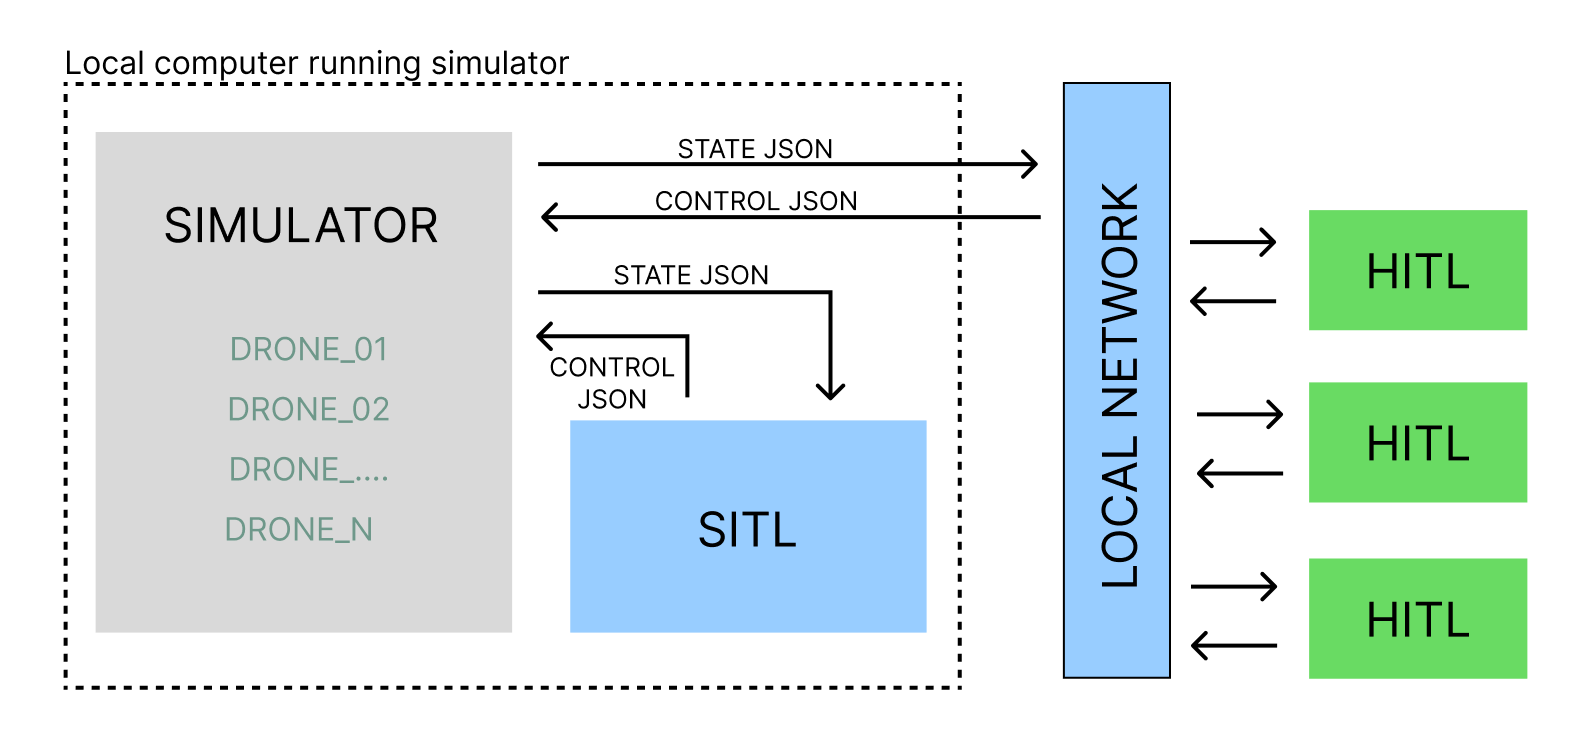
\includegraphics[width=0.8\textwidth]{images/SITL-HITL-diagram.png}
    \caption{Software-in-the-Loop and Hardware-in-the-Loop communication architecture.}
    \label{fig:sitl_hitl}
\end{figure}

 
 

 
% ── 3.5 SITL Mode ────────────────────────────────────────────────
\subsection{SITL Operation}
 
In SITL mode the controller executable runs on the same machine as simulator.
Each drone agent instance opens two UDP sockets on the loopback
interface and executes a fixed-rate control loop.
Upon receiving a state packet, the controller immediately computes and
transmits a command response, achieving a round-trip latency bounded by the
OS loopback stack (typically 1ms on Linux).
 
 
% ── 3.6 HITL Migration ───────────────────────────────────────────
\subsection{HITL Migration Path}
 
Transitioning from SITL to HITL requires modifications to only two files. 
The control logic, packet definitions, and configuration parameters remain identical across both modes.
 

\noindent The network topology changes from loopback to WiFi (IEEE 802.11),
introducing additional latency of approximately 5ms
on a local network. Given the low control bandwidth of surface vessels and the robustness of the communication protocol, this increase is well within acceptable limits for real-time control.


\section{Default drone parameters}

During all tests I used drones with the following parameters:


\begin{itemize}
    \item Mass: XXXkg
    \item Length: 3.0 m
    \item Maximum thrust: XXX N per motor
    \item Battery capacity: XXXX mAh
    \item Propeller diameter: XXX inches
    \item Control frequency: 200 Hz
    \item Sensor suite: IMU, GPS, magnetometer
    \item MORE PARAMETERS TO BE ADDED
\end{itemize}

As a 3D mocel, I used the ONR Tumblehome, designed for the ONR Tumblehome Challenge \cite{W2025_ONRT}. The model was obtained from the W2025 website and adapted for use in simulator. 



\section{AIS - Automatic Identification System}

The Automatic Identification System (AIS) is an automated tracking system used by vessels for identifying and locating ships. By electronically exchanging data with other nearby ships, AIS base stations, and satellites, it provides a real-time digital picture of maritime traffic, which is essential for collision avoidance and maritime domain awareness.

\subsection{Transmission Mechanism}

AIS operates in the VHF maritime band. It primarily uses two dedicated frequencies to manage high traffic volume and prevent signal interference:

\begin{itemize}
    \item AIS 1: 161.975 MHz
    \item AIS 2: 162.025 MHz
\end{itemize}

Because AIS is a brodcast system, it is inherently unidirectional and does not require a handshake or connection establishment. Each vessel continuously transmits its information, which can be received by any nearby AIS-equipped receiver within range.

To prevent collisions of messages in busy areas, AIS uses a dynamic slot allocation mechanism. Each vessel monitors the channel and selects an available time slot for its transmission. If a vessel detects that its chosen slot is occupied, it will randomly select another slot, ensuring efficient use of the VHF spectrum even in congested maritime environments.

Reporting intervals for AIS transmissions vary based on the vessel's status and speed, as defined in ITU-R M.1371-5. For example, a vessel at anchor may transmit every 3 minutes, while a vessel underway at high speed may transmit every 2 seconds. This adaptive reporting ensures that information is updated more frequently when the vessel is in motion or changing course, while conserving bandwidth when stationary.

\begin{table}[h!]
\centering
\caption{AIS Reporting Intervals for Shipborne Mobile Equipment (ITU-R M.1371-5)}
\label{tab:ais_reporting_rates}
\begin{tabular}{|l|l|l|}
\hline
\textbf{Vessel Status / Speed} & \textbf{Class A (SOTDMA)} & \textbf{Class B (CS/SO)} \\ \hline
At anchor or moored & 3 min & 3 min \\ \hline
At anchor or moored & 10 s & 3 min \\ \hline
0--14 knots & 10 s & 30 s \\ \hline
0--14 knots (changing course) & 3 1/3 s & 30 s \\ \hline
14--23 knots & 6 s & 15 s \\ \hline
14--23 knots (changing course) & 2 s & 15 s \\ \hline
$>$ 23 knots & 2 s & 5 s \\ \hline
$>$ 23 knots (changing course) & 2 s & 5 s \\ \hline
Static Information & Every 6 min & Every 6 min \\ \hline
\end{tabular}
\end{table}


\vspace{0.5cm}

Range of system is typically 20 to 30 nautical miles, depending on antenna height and atmospheric conditions. There is a satellite variant of AIS, known as S-AIS, which allows for global coverage by receiving signals from space, but this is not the focus of this project.

\subsection{Data Transmitted}
\label{subsection:data_tx}

The information broadcast by an AIS transponder is categorized into three types:

\begin{itemize}
    \item \textbf{Static Information:} Ship name, IMO number, call sign, vessel type, and vessel dimensions (programmed at installation).
    \item \textbf{Dynamic Information:} Automatically updated data including GPS position, Course Over Ground (COG), and Speed Over Ground (SOG).
    \item \textbf{Voyage-Related Information:} Destination, estimated time of arrival (ETA), and current draught (entered manually by the crew).
\end{itemize}


\subsection{Vessel Type Classification}

\begin{longtable}{clcl}
\caption{AIS Vessel Type Codes (ITU-R M.1371)} 
\label{tab:ais-vessel-types} \\
\toprule
\textbf{Code} & \textbf{Vessel Type} & \textbf{Group} & \textbf{Notes} \\
\midrule
\endfirsthead
\multicolumn{4}{c}{\tablename\ \thetable{} -- continued} \\
\toprule
\textbf{Code} & \textbf{Vessel Type} & \textbf{Group} & \textbf{Notes} \\
\midrule
\endhead
\midrule
\multicolumn{4}{r}{\textit{Continued on next page}} \\
\endfoot
\bottomrule
\endlastfoot

0   & Not available             & Unknown  & Default / not specified \\
\midrule
\multicolumn{4}{l}{\textit{Special Purpose Ships}} \\
\midrule
01  & Science / Research vessel & Special  & \\
02  & Training vessel           & Special  & \\
03  & Government-owned vessel   & Special  & \\
04  & Ice breaker               & Special  & \\
05  & Buoy / AtoN tender        & Special  & Aids to Navigation \\
06  & Cable layer               & Special  & \\
07  & Pipe layer                & Special  & \\
09  & Special purpose ship      & Special  & No additional information \\
\midrule
\multicolumn{4}{l}{\textit{Support Vessels}} \\
\midrule
11  & FPSO vessel               & Support  & Production, Storage \& Offloading \\
12  & Fish factory ship         & Support  & \\
14  & Offshore support vessel   & Support  & \\
17  & Construction vessel       & Support  & \\
18  & Crew boat                 & Support  & \\
19  & Support vessel            & Support  & No additional information \\
\midrule
\multicolumn{4}{l}{\textit{Wing in Ground / Fishing / Special}} \\
\midrule
20  & Wing in ground (WIG)      & WIG      & \\
30  & Fishing                   & Fishing  & \\
31  & Towing                    & Tug/Tow  & \\
33  & Dredging / underwater     & Special  & \\
34  & Diving operations         & Special  & \\
35  & Military operations       & Military & \\
36  & Sailing                   & Sailing  & \\
37  & Pleasure craft            & Pleasure & Recommended for USV/drone \\
\midrule
\multicolumn{4}{l}{\textit{High Speed Craft}} \\
\midrule
40  & High speed craft (HSC)    & HSC      & All ships of this type \\
\midrule
\multicolumn{4}{l}{\textit{Special Craft}} \\
\midrule
50  & Pilot vessel              & Special  & \\
51  & Search and rescue         & Special  & SAR \\
52  & Tug                       & Tug/Tow  & \\
53  & Port tender               & Special  & \\
54  & Anti-pollution            & Special  & \\
55  & Law enforcement           & Special  & \\
58  & Medical transport         & Special  & \\
59  & Non-combatant ship        & Special  & Per RR No.\ 18 \\
\midrule
\multicolumn{4}{l}{\textit{Passenger / Cargo / Tanker / Other}} \\
\midrule
60  & Passenger                 & Passenger & All ships of this type \\
70  & Cargo                     & Cargo     & All ships of this type \\
80  & Tanker                    & Tanker    & All ships of this type \\
90  & Other                     & Other     & All ships of this type \\

\end{longtable}

\noindent\textbf{Note:} Codes x1--x4 denote hazardous cargo categories A--D, omitted for brevity.
Codes 01--19 are an extended classification outside the core ITU-R M.1371 range (20--99).\\[4pt]
\noindent\textbf{Drones / USV:} No dedicated code exists.
Use \textbf{37} (civilian), \textbf{35} (naval), or \textbf{90} (unambiguous).




\subsection{AIS Vulnerability: GPS Integration and Spoofing}

The integrity of AIS data is fundamentally dependent on the Global Navigation Satellite System (GNSS), most commonly GPS. While AIS uses VHF for the transmission of data, the "Dynamic Information" (position, speed, and course) is pulled directly from the ship’s onboard GPS receiver. This creates a critical vulnerability: if the GPS signal is compromised, the AIS broadcast becomes a vehicle for misinformation.



\begin{figure}[htbp]
    \centering
    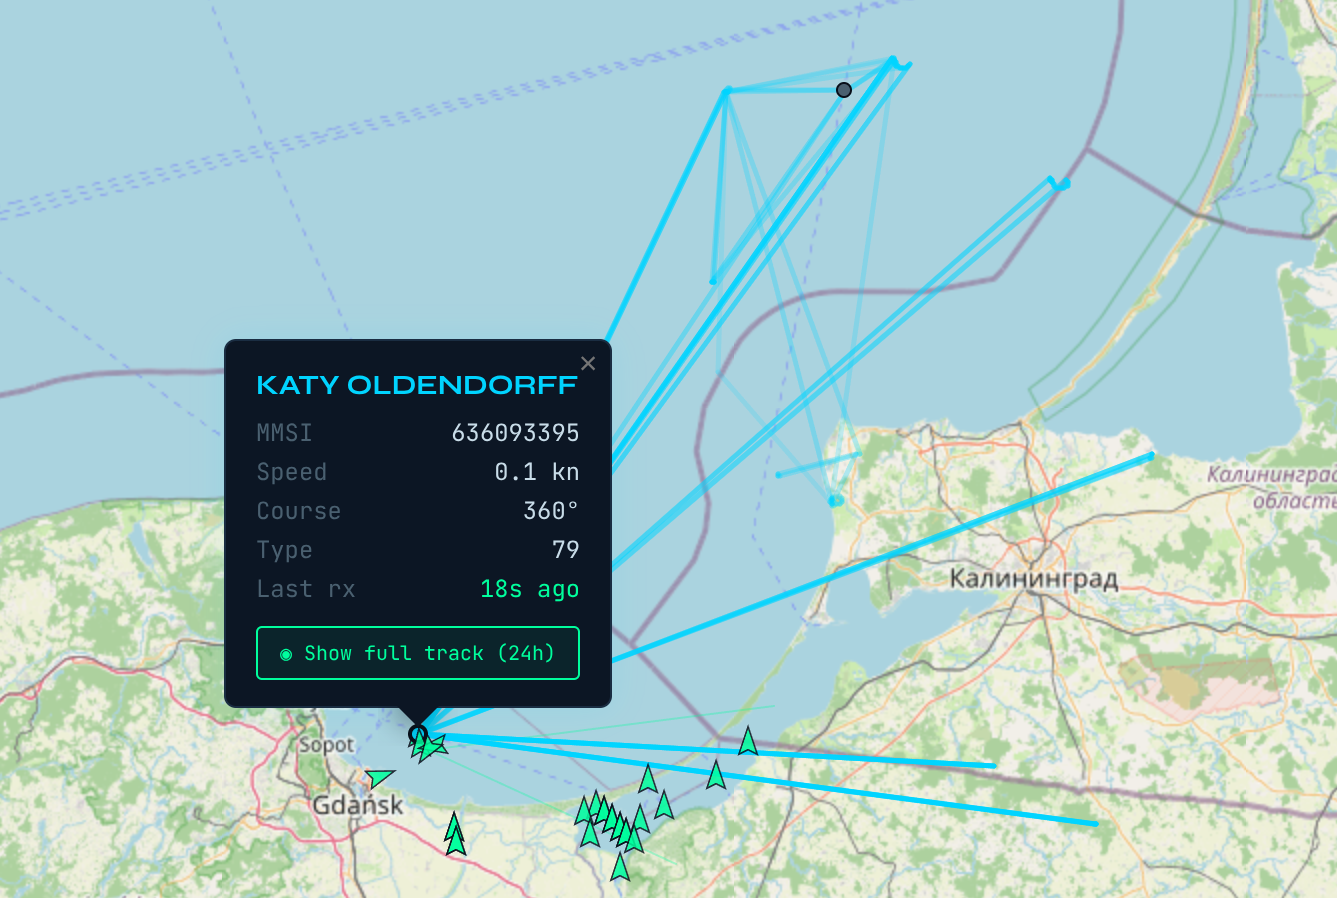
\includegraphics[width=0.6\textwidth]
    {images/AIS_GPS_SPOOF.png}
    \caption{GPS spoofing attack on a vessel, showing the compromised GPS signal.}
    \label{fig:spoofed_GPS}
\end{figure}



\subsection{Synthetic and Virtual AIS Aids to Navigation (AtoNs)}
A significant development in modern maritime infrastructure is the use of AIS signals to represent physical objects without placing electronics on the objects themselves. This is achieved through Synthetic and Virtual AIS AtoNs, which use the 99 prefix MMSI format (specifically \textbf {99MID1XXX} or \textbf {99MID6XXX}) to distinguish them from vessels.

\textbf {Synthetic AIS AtoNs}
A Synthetic AIS AtoN exists where there is a physical buoy or structure in the water, but it does not have its own AIS transmitter. Instead, a nearby AIS shore station (Base Station) broadcasts an AIS Message 21 that contains the exact coordinates of that physical buoy. This provides the mariner with a digital icon on their ECDIS/Radar that correlates with the physical object they see through the window, without the cost or maintenance of installing batteries and transmitters on every buoy.

\textbf {Virtual AIS AtoNs}
Unlike the synthetic version, a Virtual AIS AtoN marks a point where no physical buoy exists.

These are critical for "Time-Critical" marking. If a vessel sinks in a busy channel or a new hazard is discovered, authorities can instantly broadcast a Virtual AtoN to warn ships before a physical buoy can be deployed.

\section{AIS data collection}

Since the project involves simulating a maritime environment with drones, collecting real-world AIS data is crucial for creating realistic scenarios. AIS data provides information about vessel positions, speeds, and types, which can be used to populate the simulation with dynamic maritime traffic, from given time and location. This section outlines the methods for collecting AIS data, including sources, tools.

\subsection{AIS Data Sources}
Because AIS data is transmitted by vessels and received by coastal stations, there are several sources for obtaining this data:
\begin{itemize}
    \item \textbf{MarineTraffic:} A popular online platform that provides real-time and historical AIS data. It offers an paid API for accessing vessel information, which can be used to download data for specific regions and time periods.
    \item \textbf{AIS Hub:} A community-driven platform that collects AIS data from volunteers around the world. It provides free access to AIS data for research purposes, but the coverage may be limited depending on the location and the number of contributors in that area.
    \item \textbf{Local Coastal Stations:} Some coastal stations provide public access to AIS data. This can be particularly useful for collecting high-resolution data in specific areas of interest.
    \item \textbf{Homemade AIS Receiver:} Setting up a personal AIS receiver using software-defined radio (SDR) or a dedicated AIS receiver can allow for real-time data collection in the vicinity of the project location.
\end{itemize}


\begin{figure}[htbp]
    \centering
    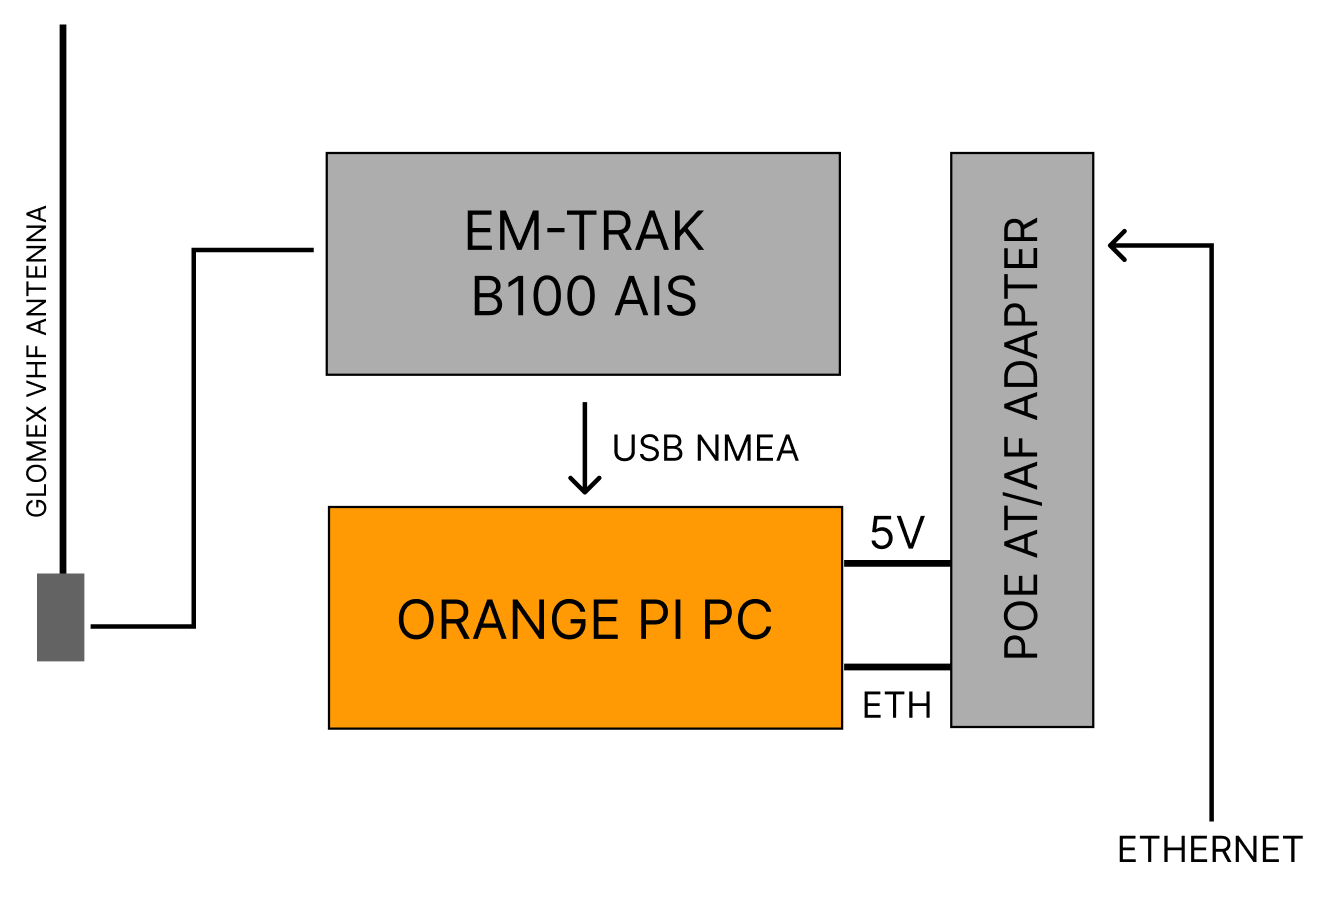
\includegraphics[width=0.6\textwidth]{images/AIS_RX_subsystems.png}
    \caption{My homemade AIS receiver system diagram.}
    \label{fig:AIS_RX_system}
\end{figure}

\vspace{0.5cm}

Since I live close to the coast, I have set up a personal AIS receiver using a
\textbf{EM-TRAK B100 AIS} receiver connected to a Orange Pi PC running custom suftware to log AIS messages, upload them to local database and visualize them on a web interface. This allows for continuous data collection and the ability to capture local maritime traffic patterns relevant to the simulation. Both AIS receiver and Orange Pi are powered by POE 802.3 at/af, which allows for easy installation and maintenance. Whole system is shown in figure \ref{fig:AIS_RX_system}. 




\vspace{0.5cm}


On a Orange Pi, I have developed a custom software that listens to the AIS receiver's output, parses the NMEA sentences, and stores the relevant data (such as MMSI, position, speed, course) in a local database. To visualize the collected AIS data, I have created a web interface that displays the positions of nearby vessels on a map in real-time. As a map I am using OpenStreetMap with Leaflet overlayer. This setup allows me to monitor maritime traffic in my area and collect data for use in the simulation environment. This system provides me a log of AIS messages in a .csv format, which can be easily imported into the simulation for creating scenarios. 

Orange Pi is running under Armbian OS, which is a lightweight Linux distribution optimized for ARM-based single-board computers. The collected AIS data is structured in a CSV format, with fields such as timestamp, MMSI, vessel name, ship type, latitude, longitude, speed in knots, and course in degrees. An example of the exported AIS data is shown in Listing \ref{lst:ais_csv_export}.

\vspace{0.5cm}

\begin{figure}[htbp]
    \centering
    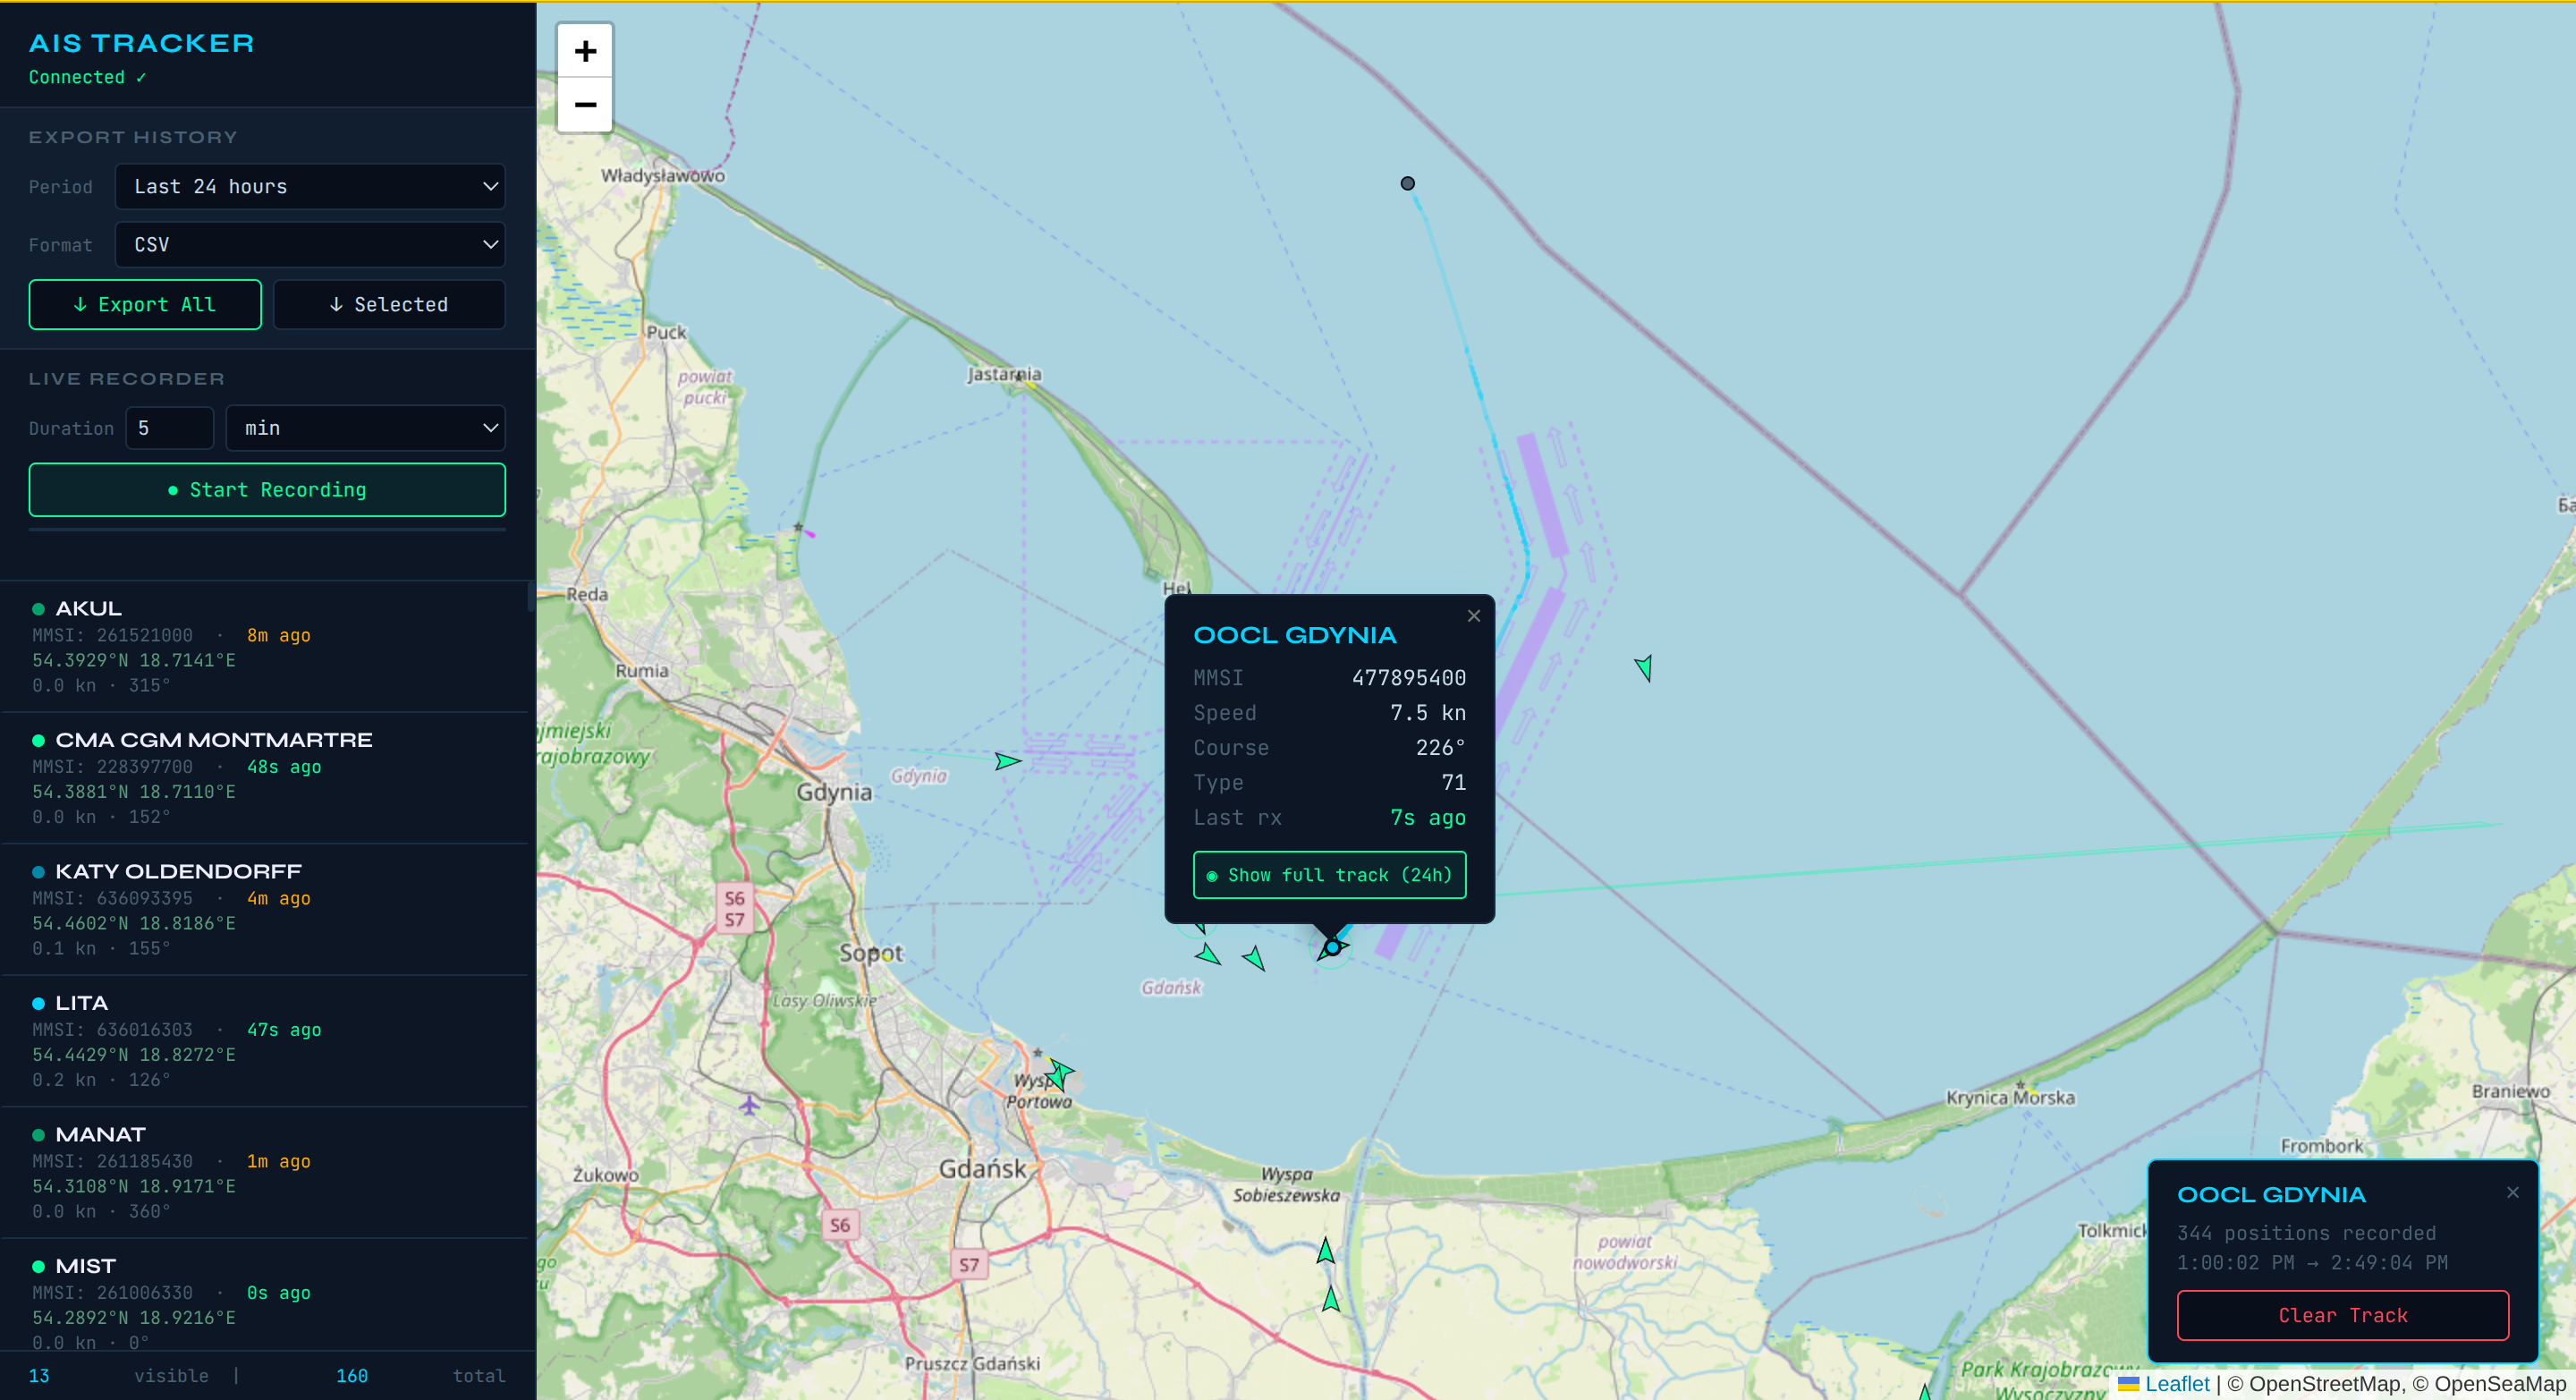
\includegraphics[width=1.0\textwidth]{images/AIS_website.png}
    \caption{My AIS data visualization web interface showing nearby vessels in real-time.}
    \label{fig:AIS_website}
\end{figure}

\vspace{0.5cm}

\subsection{Antenna and range}

To receive AIS signals I am using standard yacht VHF antenna. Model that I use is 
 \textbf {Glomex RA112}. It is a 1,5m VHF antenna with a gain of 3dB. Antenna is mounted on the roof of my house, which is approximately 10m above sea level. Between sea and my home there is a forrest, where threes might be blocking signals. With this setup, I am able to receive AIS signals from vessels within a range of approximately 20 nautical miles (37 km), depending on atmospheric conditions and the height of the transmitting vessel's antenna. This range allows me to capture a significant amount of maritime traffic in Gdańsk Bay, which is a busy shipping area. The collected data includes a variety of vessel types, speeds, and courses, providing a rich dataset for simulation.

\vspace{0.5cm}

 Listing \ref{lst:ais_csv_export}, shows the exported AIS data is structured in a CSV format. Each entry represents a received AIS message, identified by its MMSI.

\begin{lstlisting}[style=csvStyle, caption={Subsection of exported AIS telemetry for Oceania.}, label={lst:ais_csv_export}]
timestamp,mmsi,name,ship_type,lat,lon,speed_kn,course_deg
2026-04-26T06:59:51.06Z,261000150,OCEANIA,0,54.4128,19.0690,9.5,84.3
2026-04-26T07:00:12.55Z,261000150,OCEANIA,0,54.4129,19.0706,8.5,86.3
2026-04-26T07:00:32.17Z,261000150,OCEANIA,0,54.4130,19.0720,9.6,84.4
2026-04-26T07:00:42.79Z,261000150,OCEANIA,0,54.4130,19.0728,9.2,67.4
2026-04-26T07:01:01.91Z,261000150,OCEANIA,0,54.4131,19.0742,9.4,90.4
\end{lstlisting}



% Analysis and Design chapter in 'chap-analysis-and-design.tex'
%\input{chap-analysis-and-design}

% Implementation chapter in 'chap-implementation.tex'
%\input{chap-implementation}

% Conclusion chapter in 'chap-conclusion.tex'
%\input{chap-conclusion}

%\appendix

% Appendix chapter in 'chap-appendix.tex'
%\input{chap-appendix}

\bibliographystyle{plain}
\bibliography{mybibliography}

\end{document}
